\let\negmedspace\undefined
\let\negthickspace\undefined
\documentclass[journal]{IEEEtran}
\usepackage[a5paper, margin=10mm, onecolumn]{geometry}
%\usepackage{lmodern} % Ensure lmodern is loaded for pdflatex
\usepackage{tfrupee} % Include tfrupee package

\setlength{\headheight}{1cm} % Set the height of the header box
\setlength{\headsep}{0mm}     % Set the distance between the header box and the top of the text

\usepackage{gvv-book}
\usepackage{gvv}
\usepackage{cite}
\usepackage{amsmath,amssymb,amsfonts,amsthm}
\usepackage{algorithmic}
\usepackage{graphicx}
\usepackage{textcomp}
\usepackage{xcolor}
\usepackage{txfonts}
\usepackage{listings}
\usepackage{enumitem}
\usepackage{mathtools}
\usepackage{gensymb}
\usepackage{comment}
\usepackage[breaklinks=true]{hyperref}
\usepackage{tkz-euclide} 
\usepackage{listings}
% \usepackage{gvv}                                        
\def\inputGnumericTable{}                                 
\usepackage[latin1]{inputenc}                                
\usepackage{color}                                            
\usepackage{array}                                            
\usepackage{longtable}                                       
\usepackage{calc}                                             
\usepackage{multirow}                                         
\usepackage{hhline}                                           
\usepackage{ifthen}                                           
\usepackage{lscape}
\begin{document}

\bibliographystyle{IEEEtran}
\vspace{3cm}

\title{NCERT 9.1.4}
\author{EE24BTECH11036 - Krishna Patil}

% \maketitle
% \newpage
% \bigskip
{\let\newpage\relax\maketitle}

\renewcommand{\thefigure}{\theenumi}
\renewcommand{\thetable}{\theenumi}
\setlength{\intextsep}{10pt} % Space between text and floats

\textbf{Question:} Solve the ODE \((\frac{d^2y}{dx^2})^2 + \cos\left(\frac{dy}{dx}\right) = 0\)

\solution
    The given equation is:
    \[ \left(\frac{d^2y}{dx^2}\right)^2 + \cos\left(\frac{dy}{dx}\right) = 0. \]

    \begin{enumerate}
        \item \textbf{Rewrite the equation as a system of first-order ODEs.}
        Let \( v = \frac{dy}{dx} \) and \( u = \frac{d^2y}{dx^2} \). The equation becomes:
        \[ u^2 + \cos(v) = 0. \]
        From this, we solve for \( u \):
        \[ u = \pm \sqrt{-\cos(v)}, \quad \text{valid only when } \cos(v) < 0. \]

        Thus, the system of equations is:
        \begin{align*}
            \frac{dy}{dx} &= v, \\
            \frac{dv}{dx} &= u = \pm \sqrt{-\cos(v)}.
        \end{align*}

        \item \textbf{ Solve numerically using the RK4 method.}
        Using the RK4 formula, we compute successive values of \( y \), \( v \), and \( u \) iteratively:
        \begin{align*}
            k_1^y &= h \cdot v, \\
            k_1^v &= h \cdot \left(\pm \sqrt{-\cos(v)}\right), \\
            k_2^y &= h \cdot \left(v + \frac{k_1^v}{2}\right), \\
            k_2^v &= h \cdot \left(\pm \sqrt{-\cos\left(v + \frac{k_1^v}{2}\right)}\right), \\
            k_3^y &= h \cdot \left(v + \frac{k_2^v}{2}\right), \\
            k_3^v &= h \cdot \left(\pm \sqrt{-\cos\left(v + \frac{k_2^v}{2}\right)}\right), \\
            k_4^y &= h \cdot \left(v + k_3^v\right), \\
            k_4^v &= h \cdot \left(\pm \sqrt{-\cos\left(v + k_3^v\right)}\right).
        \end{align*}
        The updated values are:
        \begin{align*}
            y_{n+1} &= y_n + \frac{1}{6}\left(k_1^y + 2k_2^y + 2k_3^y + k_4^y\right), \\
            v_{n+1} &= v_n + \frac{1}{6}\left(k_1^v + 2k_2^v + 2k_3^v + k_4^v\right).
        \end{align*}

        \item \textbf{ Numerical Implementation.}
        For a numerical solution, choose initial values \( y(0) = y_0 \) and \( v(0) = v_0 \), and iterate using the formulas above.
    \end{enumerate} \\

\textbf{Explanation of the Runge-Kutta Method:}

    The Runge-Kutta method is a powerful numerical technique for solving ordinary differential equations (ODEs). It is particularly effective for approximating solutions to initial value problems of the form:
    \[ \frac{dy}{dx} = f(x, y), \quad y(x_0) = y_0. \]

    In this document, we focus on the 4th-order Runge-Kutta method (RK4), which is given by the iterative formula:
    \[ y_{n+1} = y_n + \frac{1}{6}(k_1 + 2k_2 + 2k_3 + k_4), \]
    where
    \begin{align*}
        k_1 &= h \cdot f(x_n, y_n), \\
        k_2 &= h \cdot f\left(x_n + \frac{h}{2}, y_n + \frac{k_1}{2}\right), \\
        k_3 &= h \cdot f\left(x_n + \frac{h}{2}, y_n + \frac{k_2}{2}\right), \\
        k_4 &= h \cdot f(x_n + h, y_n + k_3).
    \end{align*}

    Here, \( h \) is the step size, and \( x_n \) and \( y_n \) are the values of \( x \) and \( y \) at the \( n \)-th step.

    \begin{enumerate}
        \item \textbf{Procedure for the RK4 Method:}
            \begin{enumerate}
                \item Choose the step size \( h \).
                \item Compute \( k_1, k_2, k_3, \) and \( k_4 \) as defined above.
                \item Update \( y_{n+1} \) using the RK4 formula.
                \item Repeat for the desired number of steps or until the solution reaches a specified \( x \)-value.
            \end{enumerate}

        \item \textbf{Conclusion:}
        The Runge-Kutta method is a robust numerical tool for solving systems of ODEs, including complex equations like \((\frac{d^2y}{dx^2})^2 + \cos\left(\frac{dy}{dx}\right) = 0\). By converting the second-order ODE into a system of first-order ODEs, the method can be applied systematically to obtain an approximate solution.
    \end{enumerate}
    \newpage
Below is the plot \figref{fig:example}
\begin{figure}[h]  % The 'h' means 'here' (positioning)
    \centering  % Centers the figure
    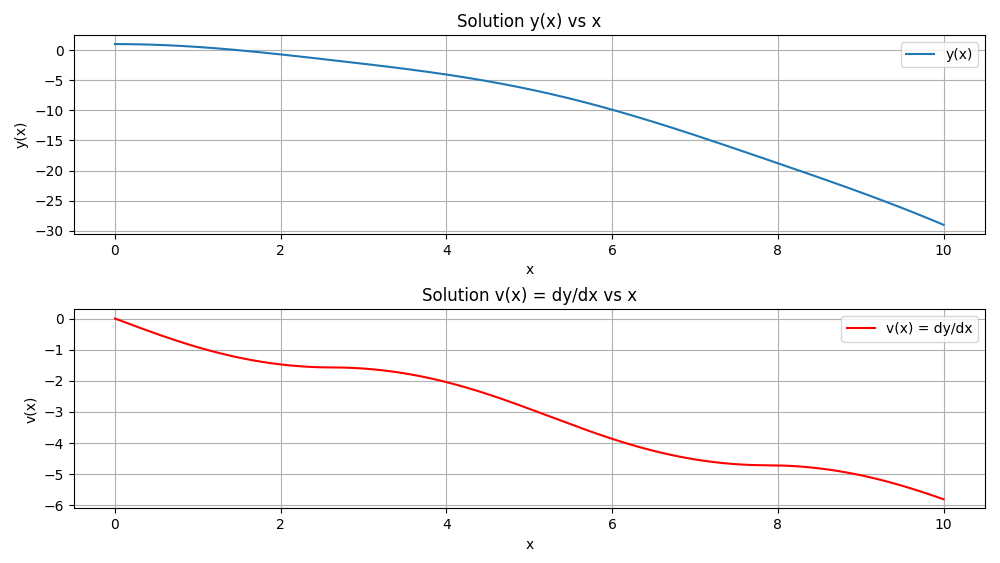
\includegraphics[width=\columnwidth]{fig/Figure_1.png}  
    \caption{Verification}
    \label{fig:example}  % Label for referencing
\end{figure}


\end{document}
